
\subsubsection{Polinomi con coefficienti discordi}
Si consideri il seguente polinomio
$$
p(s) = s^5 + 8s^4 + 17s^3 + 8s^2 -14s - 10
$$
La condizione necessaria non è soddisfatta, il polinomio non può rappresentare
un sistema asintoticamente stabile, esisteranno delle radici la cui parte reale
sarà maggiore o uguale a zero.
Si costruisce comunque la tabella di Routh per esercizio e per contare il
numero di radici positive.
\begin{table}[h]
$$
\begin{array}{c:c|ccc}
& 5 & 1 & 17 & -4 \\
p & 4 & 8 & 8 & -10 \\ \hline
p & 3 & 16 &-23/2 \\
p & 2 & 55/4 & -20 \\
p & 1 & 259/22 \\
c & 0 & -20
\end{array}
$$
\end{table}
Sono presenti quattro permanenze di segno consecutive mentre il passaggio dalla
riga 1 alla riga 0 contiene una variazione di segno. Il polinomio avrà una sola
radice a parte reale positiva, la presenza del termine noto -10 esclude la
presenza di uno zero a parte reale nulla.
Risolvendo il polinomio con un calcolatore si ottiene:
$$
\lambda_i = \{ -5,-2,-1\pm j,1 \}
$$

\subsubsection{Ulteriore esempio}
Anche in questo caso non è soddisfatta la condizione necessaria
$$
p(s) = s^4 - 6s^3 - 11s^2 + 74 s + 78
$$
Si applica la tabella di Routh
$$
\begin{array}{c:c|ccc}
&4 & 1 & -11 & 78\\
c&3 & -6 & 74 \\ \hline
c&2 & 4/3 & 78 \\
p&1 & 425 \\
p&0 & 78
\end{array}
$$
Il polinomio ha due radici a parte reale negativa e due a parte reale maggiore
o uguale a zero
$$
\lambda_i = \{-3,-1,5\pm j\}
$$

\newpage
\subsubsection{Tabella contenente uno zero}
Si analizza il seguente polinomio
$$
p(s) = s^4 + s^3 + s^2 + s + 2
$$
È soddisfatta la condizione necessaria ma nella costruzione della tabella
compare uno zero, dunque non è ben definita e il polinomio non ammette tutte le
soluzioni a parte reale negativa.
$$
\begin{array}{c:c|cccc}
 & 4 & 1 & 1 & 2 \\
 & 3 & 1 & 1 \\ \hline
 & 2 & 0  \\
 & 1 \\
 & 0
\end{array}
$$

Se si volesse comunque contare il numero di zeri a parte reale positiva e
negativa esistono alcune tecniche equivalenti per continuare il calcolo.

\textbf{Tecnica delle perturbazioni elementari}

Si può sommare una $\varepsilon$ infinitesima positiva ai coefficienti, ossia
perturbarli localmente per eliminare lo zero, si continua lo sviluppo della
tabella:
$$
\begin{array}{cc:c|cccc}
\varepsilon<0 & \varepsilon>0  & 4 & 1 & 1 & 2 \\
p & p & 3 & 1 & 1 \\ \hline
c & p & 2 & \varepsilon & 2  \\
c & c & 1 & -2/\varepsilon\\
p & c & 0 & 2
\end{array}
$$
Il primo elemento sotto lo zero sarà
$$
c_{1,1} = -\frac{1}{\varepsilon}\begin{vmatrix}
1 & 1 \\
\varepsilon & 2
\end{vmatrix} = -\frac{1}{\varepsilon}(2-\varepsilon) \simeq
-\frac{2}{\varepsilon}
$$
Con $\varepsilon$ infinitesimo positivo si hanno due permanenze e due cambi di
segno, se $\varepsilon$ fosse negativo invece si vede che il risultato non
cambia.
Questa tecnica è valida se si azzera un elemento in prima colonna ma non
più di uno zero per riga.

\newpage
\subsubsection{Zeri multipli sulla stessa riga}
Si consideri una riga $i$-esima contenente più di uno zero tra i primi $p$
elementi, si moltiplicano i coefficienti della riga per $(-1)^p$,
successivamente si trasla la riga verso sinistra di $p$ posizioni eliminando
gli zeri, si somma questa nuova riga più piccola ottenuta e la si somma alla
riga $i$-esima originale; il risultato della somma viene sostituito al posto
della riga $i$-esima.


Si applica la tecnica al polinomio precedente, si vede che $p=1$, la riga 2
$(0,\ 2)$ viene moltiplicata per $-1$ e traslata di una posizione a sinistra
ottenendo $(-2,\ 0)$, successivamente sommata alla riga iniziale, si ottiene la
nuova tabella
$$
\begin{array}{c:c|cccc}
   & 4 & 1 & 1 & 2 \\
 p & 3 & 1 & 1 \\ \hline
 c & 2 & -2 & 2  \\
 c & 1 & 2 \\
 p & 0 & 2
\end{array}
$$

Un'ulteriore tecnica prevede di moltiplicare il polinomio per una radice nota,
aumentandone il grado, si ricostruisce la tabella di Routh, non dovrebbe
comparire più lo zero nella prima colonna, salvo casi eccezionali, se ciò non
dovesse accadere si può cambiare il valore della radice. Si dovrà togliere
successivamente al numero di radici positive o negative quella aggiunta
arbitrariamente, in base al suo segno.

\subsubsection{Annullamento di un'intera riga}
Si consideri il polinomio
$$
p(s) = s^5 + s^4 + s^3 + s^2 + s + 1
$$
La condizione necessaria è verificata, si costruisce la tabella di Routh, tutta
la riga 3 sarà nulla
$$
\begin{array}{c:c|ccc}
  & 5 & 1 & 1 & 1 \\
p & 4 & 1 & 1 & 1 \\ \hline
  & 3 & 0 & 0 \\
  & 2 \\
  & 1 \\
  & 0
\end{array}
$$
In questo caso il polinomio di partenza può essere fattorizzato in un prodotto
di due polinomi $p'(s) \cdot p''(s)$, il primo polinomio dipende da tutte le
righe della tabella di Routh fino a quella prima della riga nulla, in questo
caso 5 e 4. Un'intera riga si può annullare solo in posizioni dispari (3).
Le radici contenute nel polinomio $p'$ rispettano la permanenza di segno delle
righe precedenti a quella annullata, di conseguenza in questo caso il polinomio
$p'$ avrà una sola radice con parte reale negativa.
Le restanti righe riguardano il polinomio $p''$, sarà di ordine pari al numero
di righe rimanenti, è di ordine sempre pari ed è biquadratico, ossia scrivibile
nella forma $s^2$.

Le radici di un polinomio biquadratico hanno sempre simmetria quadrantale, una
radice reale avrà una radice simmetrica sull'asse reale di segno opposto, una
coppia di radici complesse e coniugate avranno un'altra coppia sul lato opposto
rispetto all'asse reale; ogni quadrante ha la stessa disposizione delle
radici, si ottiene ruotando quello adiacente.

Sicuramente la condizione necessaria di Routh non è soddisfatta, avrà solo i
coefficienti delle potenze pari mentre quelli delle potenze dispari saranno
nulli, in ogni caso non potrebbero esistere radici che non appartengano almeno
all'asse immaginario o siano a parte reale positiva.

I coefficienti del polinomio $p''$ sono quelli dell'ultima riga prima prima
della riga nulla
$$
p''(s) = s^4 + s^2 + 1
$$
Si potrebbe ottenere il polinomio $p'$ eseguendo una divisione
$$
\polylongdiv[style=D,vars=s]{s^5+s^4+s^3+s^2+s+1}{s^4+s^2+1}
$$
Più rapidamente si può ottenere la riga mancante in tabella derivando il
polinomio $p''$ ed inserendo i coefficienti ottenuti $\frac{dp''(s)}{ds} = 4s^3
+ 2s$.

La nuova tabella ottenuta sarà
$$
\begin{array}{c:c|ccc}
  & 5 & 1 & 1 & 1 \\
p & 4 & 1 & 1 & 1 \\ \hline
p & 3 & 4 & 2 & \frac{dp''}{ds}\\
p & 2 & 2 & 4 &(\times 4)\\
c & 1 & -12 & & (\times2)\\
c & 0 & 4
\end{array}
$$
Il polinomio $p''$ avrà due radici a parte reale negativa e due a parte
reale positiva.

\newpage
\subsection{Studio dei sistemi a parametri incerti}
Un sistema è a parametri incerti se alcuni suoi parametri sono forniti con un
intervallo di incertezza oppure non sono ancora stati dimensionati, ad esempio
il sistema può contenere dei regolatori a struttura preassegnata come i
regolatori ``PID'' (\textit{Proporzionali-Integrali-Derivativi}) la cui
struttura e consecutiva legge di controllo sono già assegnati, vanno solo
impostati i giusti parametri.
Si cerca dunque la regione di asintotica stabilità (RAS) nell'insieme dei
parametri, il criterio di Routh si presta bene a questi studi.

Si consideri il polinomio
$$
p(s) =s^3 + (2+\beta)^2s^2 + (1+2\beta)s + \alpha + \beta \qquad \alpha,\beta
\in \mathbb{R}
$$

Si deve sempre imporre la condizione necessaria
$$\left\{\begin{aligned}
2+\beta &> 0 \\
1+2\beta &> 0 \\
\alpha+ \beta &> 0
\end{aligned}\right.\Rightarrow
\left\{\begin{aligned}
&\cancel{\beta  > -2}\\
&\beta  > -\frac{1}{2} \\
&\beta  > -\alpha
\end{aligned}\right.
$$
Con soli due parametri è possibile rappresentare graficamente questa regione,
la RAS è sicuramente contenuta in questa regione, potrebbe essere però più
piccola. Per individuare la RAS si costruisce la tabella di Routh, i
coefficienti della prima colonna devono avere tutti lo stesso segno
$$
\begin{array}{c|cc}
3 & 1 & 1+2\beta \\
2 & 2+\beta & \alpha + \beta \\ \hline
1 & \frac{2(\beta+1)^2-\alpha}{2+\beta}\\
0 & \alpha+\beta
\end{array}\Rightarrow\left\{
\begin{aligned}
&2+\beta > 0 \\
&\frac{2(\beta+1)^2-\alpha}{2+\beta} > 0\\
&\alpha + \beta > 0
\end{aligned}\right.\Rightarrow
\left\{\begin{aligned}
&\beta>-2\\
&2(\beta+1)^2 > \alpha\\
&\beta > -\alpha
\end{aligned}\right.
$$
Intersecando i due sistemi ottenuti si ottiene la RAS
\begin{figure}[h]
 \centering
 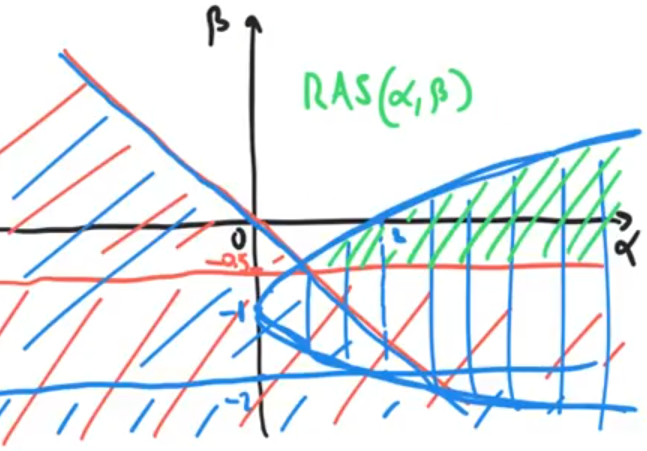
\includegraphics[width=\picwid]{ras_alpha_beta}
\end{figure}

\newpage
\subsubsection{Criterio di Karithonov}
Il criterio di Karithonov fa uso del criterio di Routh per risolvere il
problema di un sistema definito da parametri con una certa tolleranza.

Si consideri un polinomio definito dalla seguente lista di coefficienti
compresi in un certo intervallo di valori:
$$
P(s) : \{\alpha_0,\alpha_1,\alpha_2,\ldots,\alpha_n\} \qquad
\alpha_i\in[\alpha_i^-,\alpha_i^+]\quad i=0,\ldots,n
$$

È un caso tipico di tutti i sistemi i cui parametri sono forniti dal
costruttore con una tolleranza oppure sono stati studiati mediante un certo
strumento con un'accuratezza finita o ancora sono sottoposti a temperature
molto diverse tra loro e i loro parametri hanno una certa dipendenza dalla
temperatura.

Al fine di studiare l'asintotica stabilità vengono costruiti quattro polinomi
utilizzando gli estremi di ogni parametro secondo uno specifico ordine
$$
\begin{aligned}
P_a(s) &:
\{\alpha_0^+,\alpha_1^+,\alpha_2^-,\alpha_3^-,\alpha_4^+,\alpha_5^+,\ldots\}\\
P_b(s) &:
\{\alpha_0^-,\alpha_1^-,\alpha_2^+,\alpha_3^+,\alpha_4^-,\alpha_5^-,\ldots\}\\
P_c(s) &:
\{\alpha_0^+,\alpha_1^-,\alpha_2^-,\alpha_3^+,\alpha_4^+,\alpha_5^-,\ldots\}\\
P_d(s) &:
\{\alpha_0^-,\alpha_1^+,\alpha_2^+,\alpha_3^-,\alpha_4^-,\alpha_5^+,\ldots\}
\end{aligned}
$$
Il polinomio $P_b$ è il negato (nel senso dei segni) di $P_a$, il polinomio
$P_c$ ha i segni traslati di una posizione verso sinistra rispetto a $P_a$, il
polinomio $P_c$ è il negato (nel senso dei segni) di $P_a$.

Il criterio di Karithonov garantisce che il polinomio di partenza $P(s)$ abbia
tutte radici a parte reale negativa, per qualunque combinazione di valori di
$\alpha$ compresi nei rispettivi intervalli prima definiti se i quattro
polinomi costruiti hanno tutti radici a parte reale negativa, si applica il
criterio di Routh ad ogni singolo polinomio.

\subsection{Legame tra stabilità asintotica e funzione di trasferimento}
Un sistema è stabile se la sua funzione di trasferimento converge
asintoticamente a zero, questo tipo di stabilità prende il nome di stabilità
esterna o ingresso-uscita, chiamata anche \textit{BIBO}
Bounded-Input-Bounded-Output o \textit{LILO} Limited-Input-Limited-Output.

La stabilità secondo Liapunov è invece un concetto di stabilità interna al
sistema, locale nell'intorno del punto di equilibrio. È comunque un concetto di
stabilità più forte perché riguarda lo stato del sistema e implica quella
esterna, se i modi del sistema, studiati con il criterio di Liapunov, sono
convergenti allora lo saranno sicuramente quelli eccitabili ed osservabili,
analizzati dalla funzione di trasferimento.

L'implicazione inversa è vera solo per i sistemi in forma minima, ossia se
tutti i suoi modi sono raggiungibili (eccitabili) ed osservabili.
La matrice esponenziale $e^{At}$ può essere espressa come rapporto tra una
matrice $E(s)$ e un polinomio $m(s)$. Si applica l'impulso, ovvero si
moltiplica per le matrici $C$ e $B$ per ottenere la risposta all'impulso e si
ricava il rapporto tra una matrice $N(s)$ e un polinomio $dw(s)$ chiamato
polinomio minimo. Se il polinomio minimo coincide con il polinomio
caratteristico $P(s)=|sI-A|$, allora il sistema è in forma minima.
$$
W(t)  = Ce^{At}B = C\frac{E(s)}{m(s)}B = \frac{N(s)}{dw(s)}
$$
Nel polinomio $m(s)$ sono presenti tutti i modi, moltiplicando per $C$ e $B$
potrebbero esserci delle cancellazioni e il polinomio $dw(s)$ potrebbe non
contenere tutti i modi e il sistema non essere in forma minima.

Se il sistema è in forma ISU si costruisce la matrice $A$ e si calcola il
polinomio caratteristico, studiandolo con il criterio di Routh.
In alternativa si può costruire la funzione di trasferimento
$W(s)=\frac{N(s)}{dw(s)}$, si può utilizzare il polinomio $dw(s)$ ma devono
essere eseguite prima tutte le cancellazioni, se e solo se il polinomio ha
ancora grado $n$ allora si può utilizzare per studiare la stabilità interna.

\subsection{Metodo indiretto di Lyapunov (I criterio)}
Si vuole studiare la stabilità di un punto di equilibrio non lineare mediante
lo studio di un sistema linearizzato attorno a quel punto.

Sia il sistema non lineare con ingresso costante situato in un suo punto di
equilibrio
$$
\dot{x} =f(x,u) \qquad u(t) = \overline{u} \longrightarrow
f(\overline{x},\overline{u})=0 : \overline{x} \text{ punto di equilibrio}
$$
Si costruisce il sistema linearizzato nell'intorno dei punti di equilibrio di
cui si vuole studiare la stabilità, si introducono le variabili di variazione
$$
\delta x = x-\overline{x},\quad \delta u = u - \overline{u} \rightarrow
A=\left.\frac{\partial f(x,u)}{\partial x}\right|_{
\begin{aligned}
&u=\overline{u}\\
&x=\overline{x}
\end{aligned}}
$$
Si definisce una matrice $A$ come lo Jacobiano della funzione $f$ rispetto ad
$x$ calcolato nel punto di equilibrio, per ogni punto di equilibrio.

Il primo criterio di Lyapunov afferma che il punto di equilibrio $\overline{x}$
è asintoticamente stabile se la matrice $A$ ha tutti autovalori a parte reale
negativa.
$\overline{x}$ è instabile se la matrice $A$ ha qualche autovalore a parte reale
positiva.
Non sono presenti condizioni circa la semplice stabilità del sistema, non si
può cioè affermare nulla se la matrice $A$ ha qualche autovalore a parte reale
nulla, si ricorre in questi casi al teorema di
\href{https://it.wikipedia.org/wiki/Teorema_di_LaSalle}{LaSalle}, non si può
utilizzare questo metodo perché la stabilità dipenderebbe dai parametri
trascurati nel processo di linearizzazione.

\newpage
\section{Sistemi interconnessi}
Si consideri un sistema elettromeccanico, un motore elettrico a magneti
permanenti è un sistema che ha un ingresso elettrico e un'uscita meccanica.
Il circuito elettrico è formato da una serie R-L e un generatore di tensione
proporzionale mediante una costante $K$ alla coppia resistente e alla
velocità angolare del rotore mentre la coppia motrice è proporzionale alla
corrente che circola nella maglia tramite la medesima costante $K$.

\begin{figure}[h]
 \centering
 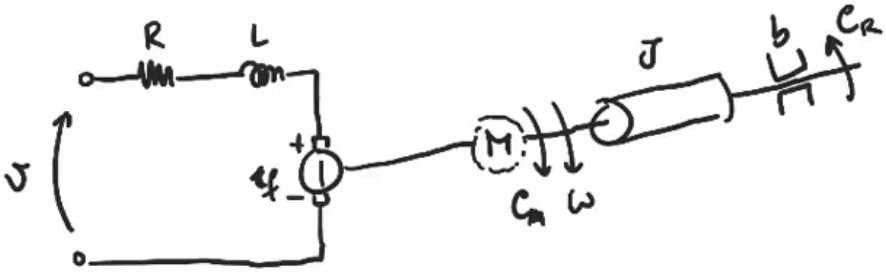
\includegraphics[width=0.6\linewidth]{motore_elettrico}
\end{figure}

Si può suddividere il sistema in un sottosistema elettrico che ha in ingresso
la tensione $v$ e la tensione $e_f$, in uscita la coppia $C_m$ che risulta
essere l'ingresso per il sistema meccanico che ha in uscita la $\omega$ oppure
ponendo un sistema integratore si otterrebbe la posizione angolare $\theta$.

\begin{figure}[h]
 \centering
 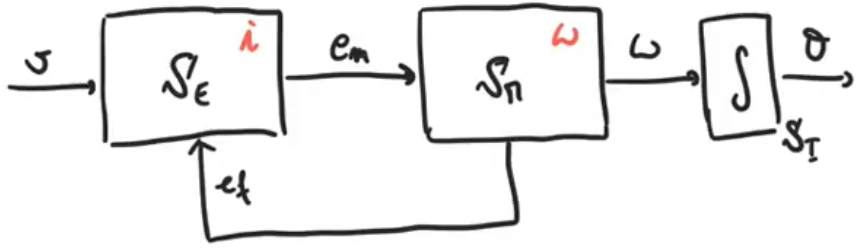
\includegraphics[width=0.6\linewidth]{motore_elettrico_schema_blocchi}
\end{figure}

Si scrive l'equazione alla maglia del sottosistema elettrico e meccanico
$$\left\{\begin{aligned}
v&=Ri+L\dot{i} + e_f \\
e_f &= K\omega
\end{aligned}\right. \qquad
\left\{\begin{aligned}
j\dot\omega &=C_m -b\omega -C_r \\
C_m &= Ki
\end{aligned}\right.
$$
Si aggiunge l'integratore
$$\left\{\begin{aligned}
\theta &= \int_0^t \omega (\tau) d\tau
\end{aligned}\right.
$$
Si costruisce la ISU del sottosistema elettrico e meccanico
$$\left\{\begin{aligned}
x_1 &= i\\
\dot{x}_1 &= -\frac{R}{L}x_1 + \frac{1}{L}v -\frac{1}{L}e_f \\
y' &= C_m = Kx_1
\end{aligned}\right. \qquad
\left\{\begin{aligned}
x_2 &= \omega \\
\dot{x}_2 &= -\frac{b}{J}x_2 + \frac{1}{J}C_m -\frac{1}{J}C_r\\
y'' &= x_2\\
y''' &= e_f = Kx_2
\end{aligned}\right.
$$
Il sottosistema integratore
$$
\left\{\begin{aligned}
 x_3 &= \theta \\
 \dot{x_3} & = \omega \\
 y &= x_3
\end{aligned}\right.
$$

Il vettore di stato complessivo è formato dall'unione di tutti gli stati
ponendo $v=u_1$ e $C_r=u_2$
$$
\left\{\begin{aligned}
\dot{x}_1 &= -\frac{R}{L}x_1 + \frac{1}{L}u_1 - \frac{K}{L}x_2 \\
\dot{x}_2 &= -\frac{b}{J}x_2 +\frac{K}{J}x_1 - \frac{1}{J}u_2\\
\dot{x}_3 & = x_2 \\
y&= x_3
\end{aligned}\right.
$$
Il sistema ISU complessivo è stato costruito tenendo in considerazione la
relazione di interconnessione tra i sistemi e le rispettive variabili che
permettono la loro interazione.
